% -------------------------------------------------------------------------------------------------
%
%  Skeleton for theses at the Institute for Dynamic Systems and Control
% -------------------------------------------------------------------------------------------------
%
% FILENAME:   thesis.tex
%
% ABSTRACT:   main file for theses
%
% EXCEPTIONS: -
%
% USAGE:      !!!!!!COMPILE WITH PDFLATEX, *NOT* WITH LATEX OR TEX!!!!!!!
%
% HISTORY:    written by Sascha A. Stoeter <stoeter@iris.ethz.ch>, www.stoeter.com, 02.06.2004
%             modified by Martin Probst, 18.08.2004
%             modified by Chauncey Graetzel, 11.05.2005
%			  modified by Julian Zilly, 1.12.2017

% -------------------------------------------------------------------------------------------------

\documentclass[12pt,a4paper,twocolumn]{article}
\usepackage{idsc_article}

% -------------------------------------------------------------------------------------------------
% Add needed packages. Some generally useful packages are listed for
% your convenience.
% -------------------------------------------------------------------------------------------------
\usepackage{subfigure}                          % enable the use of subfigures
%\usepackage[bf]{caption}                       % must go after subfigure
\usepackage[thickspace,thinqspace]{SIunits}     %
\usepackage{url}

\usepackage{hyperref}                           % enable Hyperlinks in pdf/ps Docs


% -------------------------------------------------------------------------------------------------
% Some handy definition to simplify future markup changes
% -------------------------------------------------------------------------------------------------
\providecommand{\eg}{e.g.}
\providecommand{\etal}{\textit{et al.}}
\providecommand{\ie}{i.e.}

%\setlength{\textwidth}{18cm} \setlength{\oddsidemargin}{-1cm}
%\setlength{\evensidemargin}{-1cm}

% -------------------------------------------------------------------------------------------------
% Select type of thesis
% -------------------------------------------------------------------------------------------------
\renewcommand{\idscthesistype}{Studies on Mechatronics}

% -------------------------------------------------------------------------------------------------
% Set names
% -------------------------------------------------------------------------------------------------
\renewcommand{\idscauthor}{Jan-Philipp von Bassewitz}
\renewcommand{\idscadviser}{Elena Arcari}


% -------------------------------------------------------------------------------------------------
% Beginning of the main document body
% -------------------------------------------------------------------------------------------------
\begin{document}

% include all Bib-items even if they're not cited in the text
\nocite{*}

% This is the first part of the front matter. Pages appear unnumbered
% and the pages are not counted.

% Title page: set title and date preferably formatted according to
% ISO 8601
\idsctitlepage{Gaussian Processes: Methods and Applications of Propagating Uncertainty}{2020}


% This is the second part of the front matter. Pages appear with
% lowercase roman numbering. The first page number is 'i'.
\pagenumbering{roman}

% Table of contents
\newpage
\tableofcontents
\addtocontents{toc}{\vspace{.5\baselineskip}}

% List of tables
%\newpage
%\addcontentsline{toc}{section}{\protect\numberline{}{List of Tables}}
%\listoftables

% List of figures
\newpage
\addcontentsline{toc}{section}{\protect\numberline{}{List of Figures}}
\listoffigures

\clearpage
\pagenumbering{arabic}

%%%%%%%%%%%%%%%%%%%%%%%%%%%%%%%%%%%%%%%%%%%%%%%%%%%%%%%%%%%%%%%%%%%%%%%%%%%%%%%%%%%%%%%%%%%%%%%%%%%%%%%%
%%%%%%%%%%%%%%%%%%%%%%%%%%%%%% This is the main part of the thesis. Pages appear with arabic numbering. 
%%%%%%%%%%%%%%%%%%%%%%%%%%%%%%%%%%%%%%%%%%%%%%%%%%%%%%%%%%%%%%%%%%%%%%%%%%%%%%%%%%%%%%%%%%%%%%%%%%%%%%%%

% Abstract must not be longer than one page per language.
\section*{Acknowledgements}
\textit{Thanks to Elena Arcari for guiding me through this project and her patience when it came to questions on my side.\\
Thanks to Professor Zeilinger for giving me the opportunity to do my Studies on Mechatronics project at her lab.}


\addcontentsline{toc}{section}{\protect\numberline{}{Abstract}}
\markright{Abstract}
\section*{Abstract}

Gaussian Processes (GPs) are a powerful data-driven tool for approximating unknown or expensive to evaluate functions. GPs are specifically useful for time-series prediction which is for example used in control  to model dynamical systems \cite{Paper1:GP_for_MPC}. GPs ability to express the uncertainty of the relative prediction renders them especially useful here.  GPs come with the downside that their computational effort does not scale well with large amounts of data. They are additionally difficult to evaluate at random inputs as there is no closed-form solution for such evaluations \cite{Paper2:UncertainInputPredictions}. Unfortunately the conventional ways of approximating the propagation of uncertainty underestimate it. Both of these drawbacks are reducing the applicability of GPs in control. We will address this issue in the following report by summarizing a range of recent state-of-the-art solutions to these challenges.


% Main body
\section{Introduction}
\label{s:Introduction}
We will start by introducing the mathematics behind Gaussian Processes and the respective function-space and weight-space interpretations. After introducing the mathematics and giving an intuition for the assumptions underlying the formulation, the report will continue by focusing on the evaluation at stochastic inputs, which will result in an expression for a probability distribution of which no closed form solution exists \cite{Paper2:UncertainInputPredictions,Paper3:GPPriorsWithUncertainInputs}. \newline

Solving this equation numerically is computationally infeasible. This issue will then be viewed from different perspectives. Firstly we will introduce the conventional approaches of approximating the stochastic evaluations seen in \cite{Paper4:TrajecotryPrediction_Taylorexpansion} and highlight their downsides. Using a Gaussian approximation and Taylor expansion \cite{Paper2:UncertainInputPredictions} will result in relatively good approximations of the mean and variance of predictions. Alternatively approaching the problem of finding the probability distribution by sampling, will open the door for other approximations using both the function-space and weight-space interpretation \cite{Paper4:TrajecotryPrediction_Taylorexpansion}. Combining these will in the end result in satisfactory results, that significantly improve on the understatement of uncertainty and high computational burden \cite{Paper5:PriorPosteriorSplit}. In this report we will lay special focus on time-series prediction of the scalar autonomous system  
\begin{equation}
    \label{eq:scalarautonomous}
     x_{k+1} = f(x_k) + w_k  
\end{equation}
where $w$ is noise with $w \sim \mathcal N (0,\sigma_w^2)$. The summarized concepts can be formulated and used for more general cases as well though.

\section{Gaussian Process}
There are multiple ways of interpreting Gaussian Process models. In the following sections we want to highlight the function-space and weight-space interpretation which are both explained in more detail in \cite{GP_for_ML}. GPs can be applied both in regression and classification problems and stand out because of their inherent ability to associate an uncertainty measurement with every prediction.

\subsection{Function-Space Interpretation}
    In the function-space interpretation one can think of a GP as a distribution over functions, which is entirely defined by a mean function $m(x)$ and a covariance function $k(x,x')$. They are described by
        $$
        m(x) =\mathbb{E}[f(x)]
        $$
        $$
        k(x,x') = \mathbb{E}[(f(x)-m(x))(f(x')-m(x'))]
        $$
    and the GP is written as
        $$
        f({x}) \sim \mathcal{G} \mathcal{P}\left(m({x}), k\left({x}, {x}^{\prime}\right)\right).
        $$
    The prior and overall properties of this distribution depend on the covariance function. Examples of using different kernels as the covariance function and drawing function samples from the prior distribution can be seen in Figure~\ref{f:squared-exponential_prior} and Figure~\ref{f:ornstein_prior}.
    \begin{figure}[ht]
        \centering
        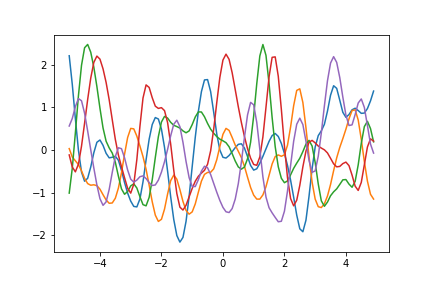
\includegraphics[width=.9\linewidth]{SoM_report_template/figures/prior.png}
        \caption[Prior with squared-exponential kernel]{\label{f:squared-exponential_prior}Function samples with squared-exponential kernel}
        \end{figure}
        \begin{figure}[ht]
        \centering
        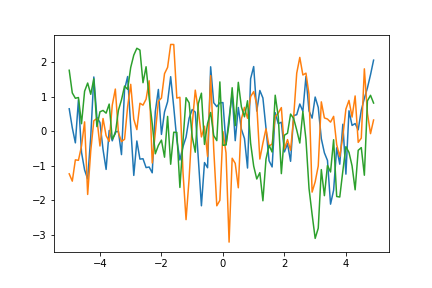
\includegraphics[width=.9\linewidth]{SoM_report_template/figures/priorornstein.png}
        \caption[Prior with Ornstein-Uhlenbeck kernel]{\label{f:ornstein_prior}Function samples with Ornstein-Uhlenbeck kernel}
    \end{figure}
    \newline
    The differences can obviously be large and the choice of $k(x,x')$ has to be made by assuming certain underlying properties of the system one would want to model. \newline
    
    To restrict the distribution over functions on functions that pass through known points the distribution can be conditioned on given data. This data consists of input values $X$ and function evaluations at these inputs $\mathbf f = f(X)$. One defines the data as $\mathcal{D}= \{\mathbf f,X\}$. This will allow drawing functions from the GP that comply with this data. An example can be seen in Figure~\ref{f:explfunction} where the known function evaluation are subject to some noise and $f(x)$ is unknown and to be found.
    \begin{figure}[ht]
        \centering
        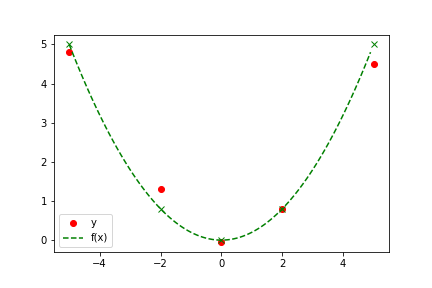
\includegraphics[width=.9\linewidth]{SoM_report_template/figures/function.png}
        \caption[Example function plot]{\label{f:explfunction}Noisy function evaluations $y$ of $f(x)=x^2$ in red.}
    \end{figure}
    To incorporate this knowledge we can write a joint Gaussian distribution between the given evaluations $\mathbb y$ and the unknown function values $\mathbb f_* := f(X_*)$. 
    \begin{equation} \begin{aligned}
    \label{eq:general_joint_gaussian}
        \footnotesize
        \setlength{\arraycolsep}{2.5pt}
        \medmuskip = 1mu % default: 4mu plus 2mu minus 4mu
        \scriptstyle
            \left[\begin{array}{c}
            \mathbf{y} \\
            \mathbf{f}_{*}
            \end{array}\right] \sim \mathcal{N}\left(\mathbf{0},\left[\begin{array}{cc}
            K(X, X)+\sigma_{n}^{2} I & K\left(X, X_{*}\right) \\
            K\left(X_{*}, X\right) & K\left(X_{*}, X_{*}\right)
            \end{array}\right]\right) \end{aligned}
    \end{equation}
    Here we inherently assume that function evaluations at \textit{close} $x$-values should result in \textit{close} function values $f(x)$. The distance is described by the covariance function $k(x,x')$ that describes how \textit{close} some points are. The term $+\sigma_{n}^{2}$ in (\ref{eq:general_joint_gaussian}) results in a covariance larger than zero for all the given function values, which implies that a certain noise is assumed in the data. This means we assume a relation $y = f(x) +\epsilon$ where $\epsilon$ is sampled from some probability density function (pdf). Setting $\sigma$ to zero will result in function samples that perfectly pass through the given data. By using the rules for finding the conditional distribution of a multivariate Gaussian one can find the mean $\mu (x)$ and variance $\Sigma(x)$ of that conditional at $x_*$ to be
    \begin{equation}
        \label{eq:GPmean}
        \mu(x_*) := 
        \mathbb{E}_{f_*}\left[\mathbf{f}_{*}|D\right] = 
        k_*^T[K+\sigma ^{2} I]^{-1} \mathbf{y}
    \end{equation}
    \begin{equation}
        \label{eq:GPvariance}
        \Sigma(x_*):=
        \mathbb{V}_{f_*}\left[\mathbf{f}_{*}|D\right] =
        k\left(x_{*}, x_{*}\right)-k_*^T\left(K+\sigma ^{2} I\right)^{-1} k_*
    \end{equation}
    where $k_* = k(x_*,X)^T$ and $K = k(X,X)$ for notational simplicity. Plotting the resultant mean and variance for the example in Figure~\ref{f:explfunction} with different kernel functions can be seen in Figure~\ref{f:interfunction}.
    \begin{figure}[ht]
        \centering
        \subfigure[Squared-exponential kernel]{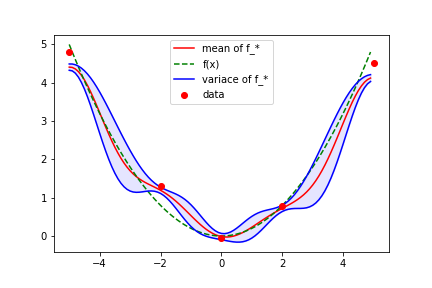
\includegraphics[width=0.9\linewidth]{SoM_report_template/figures/posterior.png}}\quad
        \subfigure[Ornstein-Uhlenbeck kernel]{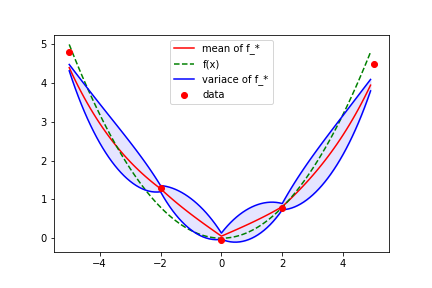
\includegraphics[width=0.9\linewidth]{SoM_report_template/figures/posteriororn.png}}
        \caption[Posterior distribution examples]{\label{f:interfunction}Posterior function distributions for different kernel functions}
    \end{figure}
    \newline
    To quantify how good the fit actually is the \textit{marginal likelihood} $p(\mathbb y|X)$ can be used. It can be computed with the integral
    $$
    p(\mathbf{y} \mid X)=\int p(\mathbf{y} \mid \mathbf{f}, X) p(\mathbf{f} \mid X) d \mathbf{f}
    $$
    that quantifies how likely the noisy measurements $y$ are as function evaluations at $X$ with the current model. Taking the logarithm allows for easier optimization and results in 
    \begin{align*}
        \log p(\mathbf{y} \mid X)=-\frac{1}{2} \mathbf{y}^{\top}\left(K+\sigma_{n}^{2} I\right)^{-1} \\ \mathbf{y}-\frac{1}{2} \log \left|K+\sigma_{n}^{2} I\right|-\frac{n}{2} \log 2 \pi
    \end{align*}
    for the GP formulation.
    \newpage
\subsection{Weight-Space Interpretation}
    As the GP describes a distribution of functions one can write it as a possibly infinite linear combination of functions. This can be written as
    \begin{equation}
        \label{eq:weight-spacef}
        f(x) = \phi(x)^T \mathbb \theta
    \end{equation}
    Sampling from the prior is easy here. It just requires sampling the required weights $\theta \sim \mathcal N (0,\Sigma_p)$. This is a property that will later in this report be of great use. The posterior can be drawn from the distribution
    \begin{equation}
        \begin{split}
        f_{*} \mid {x}_{*}, X, {y} \sim  \mathcal{N}\left(\frac{1}{\sigma_{n}^{2}} \phi\left({x}_{*}\right)^{\top} A^{-1} \Phi {y},\\ \phi\left({x}_{*}\right)^{\top} A^{-1} \phi\left({x}_{*}\right)\right).
        \end{split}
    \end{equation}
    where $\Phi = \phi(X)$ and $A = \sigma_{n}^{-2} \Phi \Phi^{\top}+\Sigma_{p}^{-1}$


\section{GP at Stochastic Inputs}
    In this section we will introduce GP evaluations at random inputs as described in \cite{Paper2:UncertainInputPredictions,Paper3:GPPriorsWithUncertainInputs}. This is important in real word applications. Sensors and actuators and therefore signals are mostly subject to noise. Assuming that the input $x_*$ is a random variable its distribution could e.g. be describes by a Gaussian distribution $x_* \sim \mathcal N(\mu_x_*, \sigma_x_*)$. The goal will be to find the distribution $\mathbb f_*$ given the distribution of $x_*$ and the data $\mathcal D$.  In the previous section the posterior distribution of $\mathbb f_*$ was introduced. Here we can write it as $p(\mathbb f_*|x_*,\mathcal D)$ where we have to assume $x_*$ to be given. By integrating over the entire input distribution one finds
    \begin{equation}
        \label{eq:posterior_distribution}
        \begin{split}
        p\left(f_{*} \mid \mu_x_*, \sigma_x_*, \mathcal{D}\right)=\\
        \int p\left(f_{*} \mid x_{*}, \mathcal{D}\right) p\left({x}_{*} \mid \mu_x_*, \sigma_x_*\right) d {x}_{*}.
        \end{split}
    \end{equation}
    Unfortunately the resultant distribution can only be evaluated numerically as no closed-form solution exists. In this section we will introduce the common ways of approximating (\ref{eq:posterior_distribution}). They can be split into multiple categories. Firstly we will introduce the ground-truth solution, followed by a procedure that uses the weight-space interpretation. Thirdly the distribution (\ref{eq:posterior_distribution}) can assumed to be Gaussian and the following mean and variance can be estimated with a Taylor expansion. Doing this jointly for the entire trajectory instead of each step iteratively will lead to decent approximation that takes the propagation of uncertainty into account.
\subsection{Ground Truth Trajectory Sampling}
    A numerical scheme proposed in \cite{Paper4:TrajecotryPrediction_Taylorexpansion} for sampling from this distribution for the scalar autonomous system case (\ref{eq:scalarautonomous}) will be presented here. It will act as a benchmark to all the other sampling based approximations following later in the text. The analogue here to the joint distribution (\ref{eq:general_joint_gaussian}) is
    \begin{equation}
        \footnotesize
        \setlength{\arraycolsep}{2.5pt}
        \medmuskip = 1mu % default: 4mu plus 2mu minus 4mu
        \scriptscriptstyle
        \centering
        \left[\begin{array}{c}
        x_{1} \\
        \vdots \\
        x_{k+1}
        \end{array}\right] \sim 
        \mathcal N \left(
        \left[\begin{array}{c}
        \mu\left(x_{0}\right) \\
        \vdots \\
        \mu\left(x_{k}\right)
        \end{array}\right] , {\left[\begin{array}{ccc}
        k\left(x_{0}, x_{0}\right)+\sigma ^2 & \ldots & k(x_0,x_k) \\
        \vdots & \ddots & \vdots \\
        k(x_k,x_0)  & \ldots & k\left(x_{k}, x_{k}\right)+\sigma ^2
        \end{array}\right]} \right).
    \end{equation}
    For a first given value $x_0$ the next step can simply be sampled from $x_1 \sim \mathcal N(\mu(x_0),k(x_0,x_0)+\sigma^2)$ with $ x_{1}=\mu\left(x_{0}\right)+\sqrt{k\left(x_{0}, x_{0}\right)+\sigma^2} \  \tilde{w}_{0} $ where $\tile{w_0}$ is drawn from a standard normal distribution. The joint distribution can then be grown one step and $x_0$ and $x_1$ sampled from it. This can be generalized to the step $k+1$ with
    \begin{equation}
    \label{eq:groundtruth}
    X_{1: k+1}=\mu\left(X_{0: k}\right)+\sqrt{k\left(X_{0: k}, X_{0: k}\right)+I \sigma^2} \tilde{W}_{0: k+1}
    \end{equation}
    where $\tilde{W}_{0: k+1}$ is drawn from a multi dimensional standard normal distribution and $\sqrt{\cdot}$ is the Cholesky decomposition. This procedure is computationally very expensive as it scales cubically $\mathcal O(N^3)$ with the prediction horizon $N$. But this approach gives accurate samples from the distribution (\ref{eq:posterior_distribution}) as no simplifying assumptions were made.
 \subsection{Approximating Samples with Basis Functions}
    The weight-space interpretation of a GP described in \cite{Paper5:PriorPosteriorSplit} serves as an interesting alternative to the function-space interpretation and can in this case be used to approximate function samples from a posterior. Let $\phi_i(x)$ be a $l$-dimensional finite set of basis functions. The GP approximation then takes the form
    \begin{equation}
        f\left({x}\right)=\sum_{i=1}^{l} \theta_i \phi_i(x).
    \end{equation}
    Inference is here done on the weight distribution of $\theta$. Choosing a prior distribution as $\theta \sim \mathcal N (0,\Sigma_p)$ the posterior distribution $\theta|y\sim \mathcal N (\mu_\theta,\Sigma_\theta)$ of the weights is described with
    \begin{equation}
        \begin{aligned}
            {\mu_\theta}&=\left({\Phi}^{\top} {\Phi}+\sigma^{2} {I}\right)^{-1} {\Phi}^{\top} {y} \\
            {\Sigma_\theta}  &=\left({\Phi}^{\top} {\Phi}+\sigma^{2} {I}\right)^{-1} \sigma^{2}.
        \end{aligned}    
    \end{equation}
    where $\Phi = \phi(X)$. Drawing from the posterior is cheap as it scales linearly with the number of function evaluations. Unfortunately this approach also underestimates the propagation of uncertainty.


\section{Gaussian Approximation with Taylor expansion}
          To simplify expression (\ref{eq:groundtruth}) the authors of paper \cite{Paper2:UncertainInputPredictions} assume the distribution to be Gaussian and compute its mean and variance. By using the law of iterated expectation values and the law of iterative variances one gets
        \begin{equation}
        \label{expGaussianApprox}
            %m(x_*) := 
            \mathbb{E}_{\mathbf{f}_*}\left[ 
            \mathbf{f}_*
            \right]
            =
            \mathbb{E}_{x_*}\left[ 
            \mathbb{E}_{\mathbf f_*}\left[\mathbf{f}_{*}|x_*\right] 
            \right]
            =
            \mathbb{E}_{x_*}\left[ 
            \mu(x_*)
            \right ]    
        \end{equation}
        \begin{equation}
        \begin{split}
        \label{varGaussianApprox}
            %v(x_*):=
            \mathbb{V}_{\mathbf{f}_*}\left[ 
            \mathbf{f}_*
            \right]
            =
            \mathbb{E}_{x_*}\left[ 
            \mathbb{V}_{\mathbf{f}_*}\left[ 
            \mathbf{f}_* | x_*
            \right]
            \right]
            +
            \mathbb{V}_{x_*}\left[ 
            \mathbb{E}_{\mathbf f_*}\left[\mathbf{f}_{*}|x_*\right] 
            \right]
            =\\
            \mathbb{E}_{x_*}\left[ 
            \Sigma(x_*)
            \right]
            +
            \mathbb{V}_{x_*}\left[ 
            \mu(x_*)
            \right].
        \end{split}
        \end{equation}
    \subsection{Independence Assumption}
        Evaluating these expressions is still not trivial. Preceding to derive a simpler expression for the scalar autonomous case  (\ref{eq:scalarautonomous}) with a first order Taylor expansion of $\mathbb{E}\left[ x_{k+1}\right ]$ and a zeroth order Taylor expansion of $ \mathbb{V}\left[ x_{k+1} \right ]$
        %$\mu(x_k) \approx \mu(\mu_{x_k}) + \nabla \mu(\mu_{x_k})(x_k - \mu_{x_k})$ 
        will yield 
        \begin{equation}
        \label{meantaylorexpofgaussianapprox}
        \begin{split}
            \mathbb{E}\left[ 
            x_{k+1}
            \right ]
            =
            \mathbb{E}\left[ 
            \mu(x_{k})
            \right ]
            +
            \mathbb{E}\left[ 
            w_k
            \right ]
            \approx \\
            \mathbb{E}\left[ 
            \mu(\mu_{x_k})+\nabla \mu(\mu_{x_k})(x_k-\mu_{x_k})
            \right ]
            =
            \mu(\mu_{x_k}).
        \end{split}
        \end{equation}
        \begin{equation}
        \label{variancetaylorexpofgaussianapprox}
        \begin{split}
            \mathbb{V}\left[ 
            x_{k+1}
            \right ]
            =
            \mathbb{E}\left[ 
            \Sigma(x_k)
            \right ]
            +
            \mathbb{V}\left[ 
            \mu(x_k)
            \right ]
            + \sigma_w^2
            \approx \\
            \Sigma(\mu_{x_k})+\sigma_w^2
            %\mathbb{V}\left[ 
            %x_{k+1}
            %\right ]
            %=
            %\mathbb{V}\left[ 
            %f(x_k)+w_k
            %right ]
            %\approx 
            %(\nabla f(\mu_{x_k}))^2 \mathbb{V}\left[ x_{k} \right ] \\
            %+ 2 (\nabla f(\mu_{x_k}))^2 Cov(x_k,w_k) 
            % \mathbb{V}\left[ 
            %_k \right ]
        \end{split}
        \end{equation}
        These equations describe the mean and variance of each of the random variables $x_i$. This can then be jointly written to lead to a naive approximation of (\ref{eq:groundtruth})
        \begin{equation}
        \label{naiveapprox}
            \footnotesize
            \setlength{\arraycolsep}{2.5pt}
            \medmuskip = 1mu % default: 4mu plus 2mu minus 4mu
            \centering
            \scriptscriptstyle
            \left[\scriptscriptstyle{\begin{array}{c}
            x_{1} \\
            \vdots \\
            x_{k+1}
            \end{array}}\right] \sim 
            \mathcal N \left(
            \left[\begin{array}{c}
            \mu\left(x_{0}\right) \\
            \vdots \\
            \mu\left(\mu_{k}\right)
            \end{array}\right] ,
            {\left[\begin{array}{ccc}
            k\left(x_{0}, x_{0}\right)+\sigma ^2 & \ldots & 0 \\
            \vdots & \ddots & \vdots \\
            0  & \ldots & k\left(\mu_{k}, \mu_{k}\right)+\sigma ^2
            \end{array}\right]} \right).
        \end{equation}
        Higher order Taylor expansions can be used for more accuracy but will increase the computational cost. Sampling from this distribution can again be done with a Cholesky similarly to (\ref{eq:groundtruth}). The sampling is cheap, does not require the iterative approach and the predictive mean is accurate. The major downside is that it underestimates the uncertainty of times-steps past the first because the propagation of uncertainty is not accounted for as can be seen from the off-diagonal parts being all zero.
    
    \subsection{Dropping the Independence Assumption}
            The same idea of linearization applied to the sampling based approach (\ref{eq:groundtruth}) is presented in \cite{Paper4:TrajecotryPrediction_Taylorexpansion}. As mentioned the first sample will be accurate with $ x_{1}=\mu\left(x_{0}\right)+\sqrt{k\left(x_{0}, x_{0}\right)+\sigma^2} \  \tilde{w}_{0} $. The following iterations will be costly due to the recalculation of the Cholesky decomposition for every time step though. So by jointly linearing $\mu(x)$ in
        \begin{equation}
        \label{twostepsgroundtruth}
        \footnotesize
        \setlength{\arraycolsep}{2.5pt}
        \medmuskip = 1mu % default: 4mu plus 2mu minus 4mu
        \centering
            \scriptscriptstyle
            \left[\begin{array}{c}
            x_{1} \\
            x_{2}
            \end{array}\right] = \left[\begin{array}{c}
            \mu\left(x_{0}\right) \\
            \mu\left(x_{1}\right)
            \end{array}\right] + \sqrt{
            \left[\begin{array}{ll}k(x_0, x_0) + \sigma ^2 & k\left(x_0, x_1\right) \\ k\left(x_1, x_0\right) & k\left(x_1, x_1\right)+\sigma ^2\end{array}\right]}
            \left[\begin{array}{c}
            \tilde{w_0} \\
            \tilde{w_1}
            \end{array}\right]
        \end{equation}
        around $\mu_1 = \mu(x_0)$ so that $\mu(x_1) = \mu(\mu_1) + \nabla \mu(\mu_1)(x_1-\mu_1)$ one gets
        \begin{equation}
        \label{linearized ground truth}
        \footnotesize
        \scriptscriptstyle
        \setlength{\arraycolsep}{0.3pt}
        \medmuskip = 1mu % default: 4mu plus 2mu minus 4mu
        \centering
            \left[\begin{array}{l}
            x_{1} \\
            x_{2}
            \end{array}\right] \approx\left[\begin{array}{c}
            \mu_{1} \\
            \mu\left(\mu_{1}\right)
            \end{array}\right]+\left[\begin{array}{cc}
            I & 0 \\
            \nabla \mu\left(\mu_{1}\right) & I
            \end{array}\right]
            \sqrt{
            \left[\begin{array}{ll}k(x_0, x_0) + \sigma ^2 & k\left(x_0, \mu_1\right) \\ k\left(\mu_1, x_0\right) & k\left(\mu_1, \mu_1\right)+\sigma ^2\end{array}\right]}
            \left[\begin{array}{c}
            \tilde{w_0} \\
            \tilde{w_1}
            \end{array}\right].
        \end{equation}
        The means $\mu_1$ and $\mu_2$ can now be used to iteratively expand the procedure to further time-steps. Generalizing the notation for N time-steps leads to 
        \begin{equation}
        \label{generalized linearization of ground truth}
            X_{1: N} \approx M_{1: N}+A \sqrt{k\left(M_{0: N-1}, M_{0: N-1}\right)+I \sigma^2} \tilde{W}.
        \end{equation}
        with $\tilde W $ being sampled from a $N $ dimensional standard normal distribution, $M = [\mu_0,...,\mu_N]^T$ and $A_{i, j}=\prod_{l=j}^{i-1} \nabla \mu\left(\mu_{l}\right)$. This approach does account for the propagating of uncertainty as can be seen in the structure of the covariance matrix which is not diagonal. It furthermore scales quadratically $\mathcal O(N^2)$ with the prediction horizon $N$ compared to the ground truth sampling which scales cubically.

\section{State-of-the-Art Approximations}
    In this section we will summarize the current state-of-the-art approximation of (\ref{eq:posterior_distribution}). A split of the posterior into the prior and an update as a function of the prior will allow for a combination of both the weight-space interpretation with its cheap evaluations of the prior and the accurate representation of the uncertainty with the function space interpretation. This will again be a sampling approach to the problem.
\subsection{Splitting Posterior}
    To combine these advantages of the weight-space interpretation and the function-space interpretation paper \cite{Paper5:PriorPosteriorSplit} introduces a split of the posterior. According to Matheron's rule one can sample from a conditional distribution $a|b$ by first sampling the two random variables $a$ and $b$ from the joint distribution and then use the update for
    $$
    ({a} \mid {b}={\beta}) ={a}+\operatorname{Cov}({a}, {b}) \operatorname{Cov}({b}, {b})^{-1}({\beta}-{b}).
    $$
    This can analogously be done for the posterior distribution of a GP with
    \begin{equation}
        \scriptstyle
        \label{eq:updatefunctionspaceview}
        \underbrace{f_* | y}_{\text {posterior}}
        =
        \underbrace{f_*}_{\text {prior}}
        +
        \underbrace{k_*^T(K+\sigma ^2I)^{-1}(y-f-\epsilon)}_{\text {update}}.
    \end{equation}
    Substituting the prior $f_*$ in (\ref{eq:updatefunctionspaceview}) with the prior from the weight-space interpretation $\phi(x)^T\theta$ where $\theta$ is sampled from a normal distribution will reduce the computational burden and not result in less accuracy. Computing the Cholesky for the prior which scales with $\mathcal O (N^3)$ with prediction horizon $N$ is not necessary anymore.
     \begin{equation}
     \label{eq:GPPosteriorSplit}
        \underbrace{f_* | y}_{\text {posterior}}
        \approx
        \underbrace{\sum_{j=1}^{l}\phi_j(x_*)\theta_j }_{\text {prior}}
        +
        \underbrace{\sum_{i=1}^{N}v_i k(x_*,x_i)}_{\text {update}}
    \end{equation}
    where $v_i$ are the components of $V = (K(X,X)+\sigma^2I)^{-1}(y-\Phi \theta -\epsilon)$. This presents a very potent approximation because it scales with $\mathcal O (N)$ and results in very accurate representations of the uncertainty which are almost identical to the ground truth. The computational burden can be reduced further by using a \textit{sparse} GP approximation with a set of $M$ inducing points \cite{Paper5:PriorPosteriorSplit}. An additional benefit is that this expression can be differentiated which is not possible for the standard GP. This is due to the fact that the prior is a linear combination of functions.

\section{Applications}
Motivating the applicability of the described methods, we would like to shortly introduce a selection of research papers that build on this research. \newline

The paper \cite{ApplicPaper1:ThompsonSamplingWithGP} on Thompson sampling uses GPs as a tool to approximate costly to evaluate or black-box functions for optimization purposes and makes use of some iterative methods described. \cite{Paper6:ThompsonSamplingWithPosteriorSplit} introduces the idea of splitting the posterior seen in (\ref{eq:GPPosteriorSplit}) to facilitate a more scalable version of Thompson sampling that makes use of the cheap and accurate sampling. \newline

On another note the papers \cite{ApplicPaper2:GPwithBackoff,ApplicPaper3:PredictionScenarios} further improve the methods of using GPs in the context of model predictive control in similar fashion to the discussed methods for the scalar autonomous case with success. 


% Conclusion
\section{Discussion}
To compare the discussed methods Figure \ref{f:Comparison} classifies them qualitatively with respect to the attributes \textit{accuracy of uncertainty propagation} and \textit{computational efficiency}. The ground-truth trajectory sampling scales cubicly but is highly accurate. The Gaussian approximation approach with Taylor expansion accounts for the propagation of uncertainty while only scaling quadratically. The computational complexity is further decreased with the independence assumption but at the cost of accuracy. The same is true for the basis function approximation that scales linearly but is again incaccurate. The posterior split method on the other hand combines an accurate representation of the uncertainty plus it only scales linearly with the prediction horizon.
\begin{figure}[ht]
        \centering
        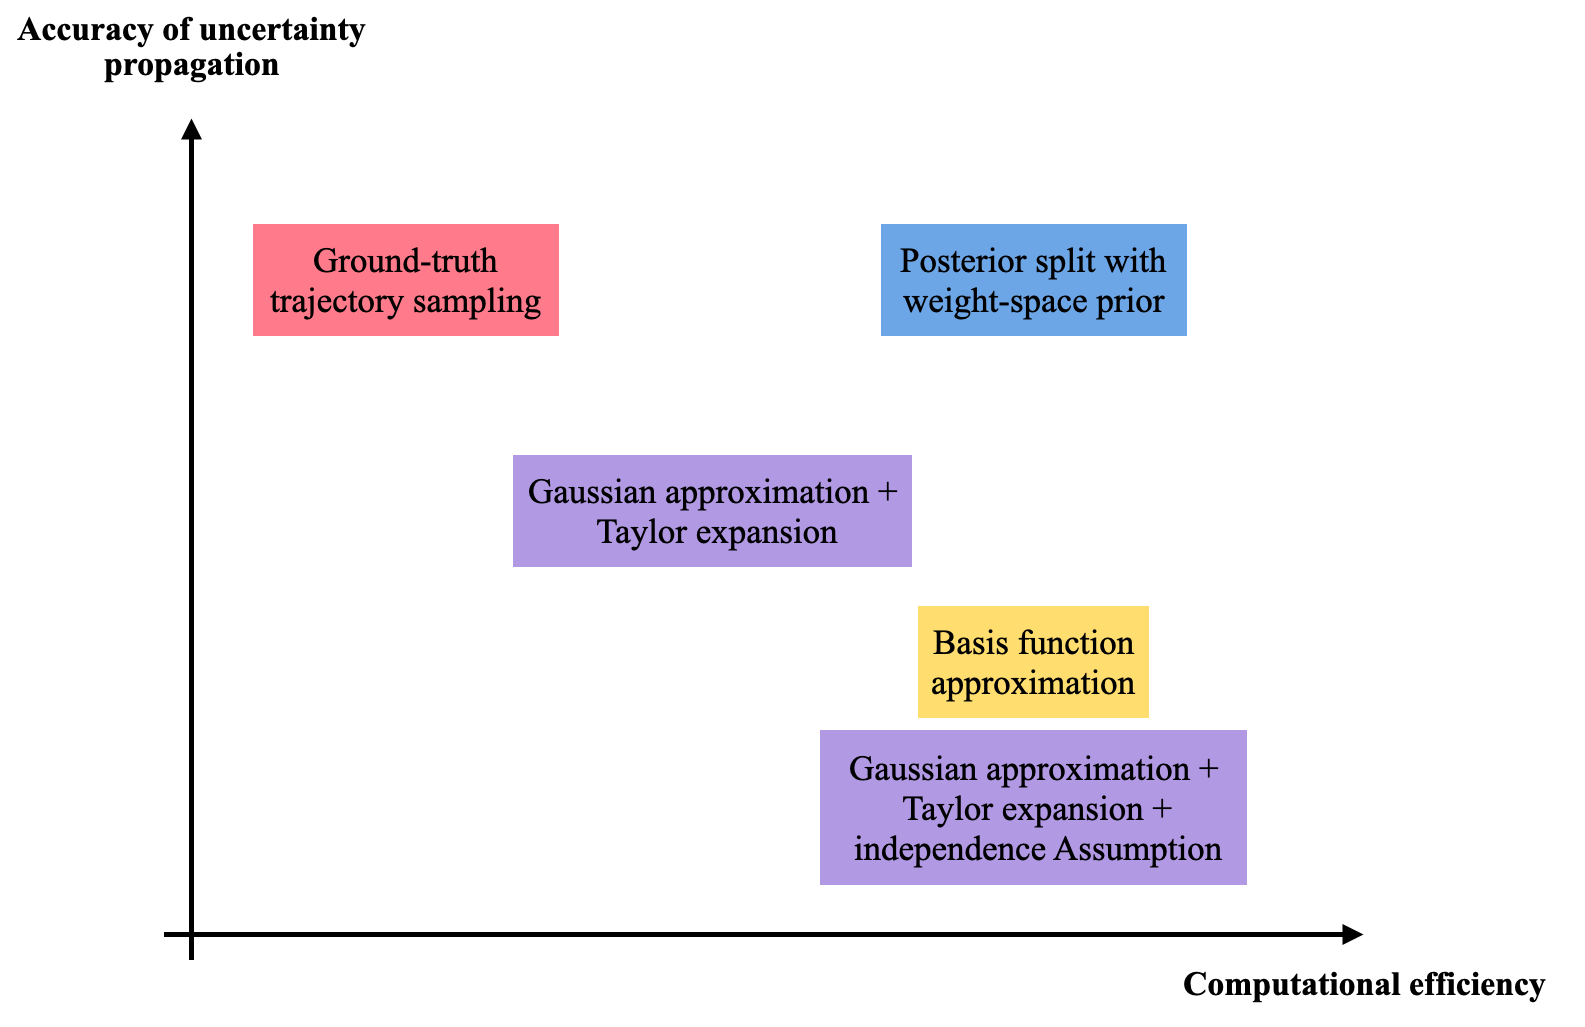
\includegraphics[width=1.1\linewidth]{SoM_report_template/figures/Bildschirmfoto 2020-12-18 um 12.50.51.png}
        \caption[Qualitative comparison of methods]{\label{f:Comparison} Qualitative comparison of methods }
\end{figure}

\section{Conclusion}
In conclusion there are many methods proposed in the literature to deal with the drawbacks of GPs, specifically lack of scalability and inaccurate approximations of uncertainty propagation. While they all improve on the naive trajectory sampling (\ref{naiveapprox}) they differ in computational cost and accuracy. The method that stands out is the combination of function-space and weight-space interpretation (\ref{eq:GPPosteriorSplit}), as it both preserves the uncertainty propagation and scales only linearly with the prediction horizon. 


% Bibliography
\newpage
\addtocontents{toc}{\vspace{.5\baselineskip}}
\addcontentsline{toc}{section}{\protect\numberline{}{References}}
\bibliography{article}


% Appendices (if needed)
%\addtocontents{toc}{\vspace{.5\baselineskip}}
%\appendix
%\section{Extra Stuff}
\label{s:ExtraStuff}

Additional material such as long mathematical derivations.

%\include{Examples}
\end{document}
